\newpage
\section{Historia del mercado laboral colombiano}

\begin{figure}[htbp]
  \centering
  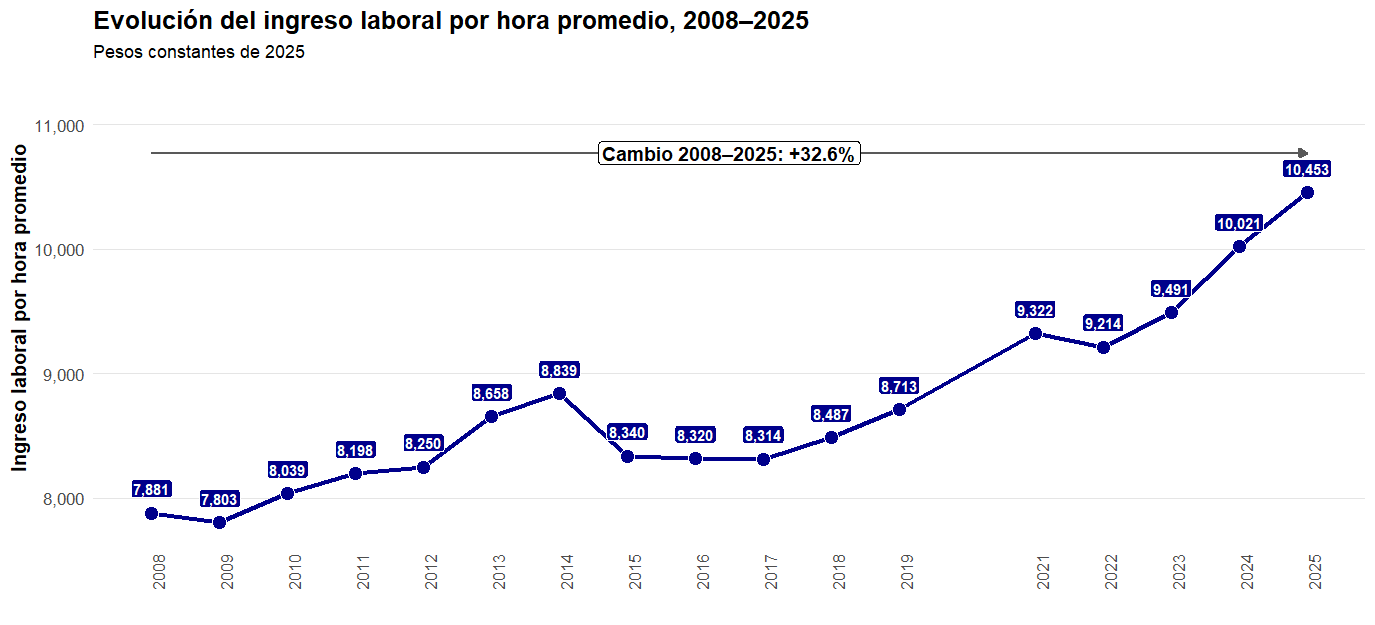
\includegraphics[width=0.9\textwidth]{Paper/figures/fig1Informe.png}
  \caption{Evolución general del ingreso laboral}
  \label{fig:1Informe}
\end{figure}

El ingreso laboral promedio por hora pasó de $7.881 en 2008 a $10.453 en 2025, un aumento real del 32,6\%. Eso es una buena noticia: los trabajadores colombianos en promedio sí ganaron más poder adquisitivo a lo largo del período.
Sin embargo, el camino no fue lineal. Hubo un primer ciclo de crecimiento hasta 2014, luego un estancamiento notable entre 2015 y 2019, y finalmente una aceleración importante a partir de 2021 que llevó los ingresos a sus niveles más altos del período. Este repunte reciente probablemente refleja una combinación de recuperación post-pandemia, ajustes al salario mínimo y cambios en la composición del empleo.

\begin{figure}[htbp]
  \centering
  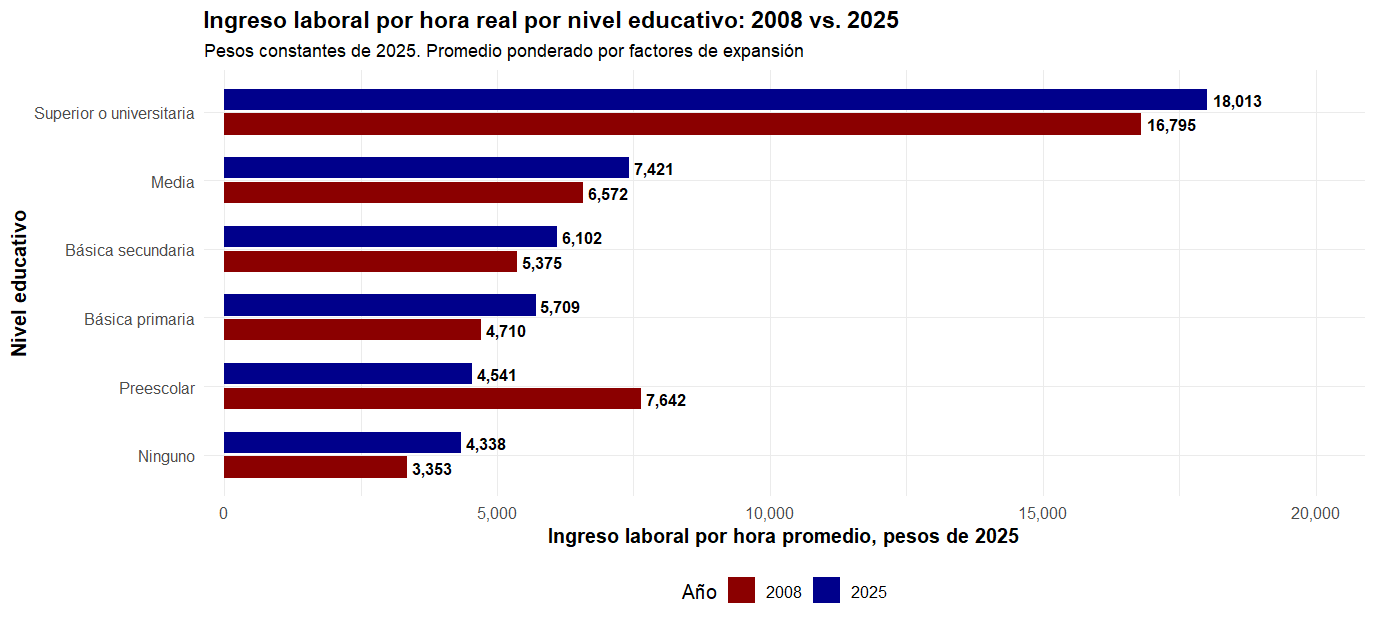
\includegraphics[width=0.9\textwidth]{Paper/figures/fig6Informe.png}
  \caption{Ingreso laboral por nivel educativo}
  \label{fig:2Informe}
\end{figure}

La educación sigue siendo el factor que más diferencia los ingresos. En 2025, un trabajador con nivel superior o universitario gana en promedio \$18.013 por hora, mientras que alguien sin ningún nivel educativo gana \$4.338, es decir, más de cuatro veces menos.
Comparando 2008 con 2025, todos los niveles educativos muestran ganancias reales, lo cual es positivo. No obstante, hay un dato curioso: los trabajadores con nivel preescolar registraron una caída en su ingreso real (de \$7.642 en 2008 a \$4.541 en 2025). Esto probablemente refleja cambios en la composición de ese grupo más que un deterioro generalizado, pero vale la pena investigarlo más a fondo.
La conclusión principal es que invertir en educación sigue siendo la palanca más poderosa para mejorar los ingresos laborales en Colombia.

\begin{figure}[htbp]
  \centering
  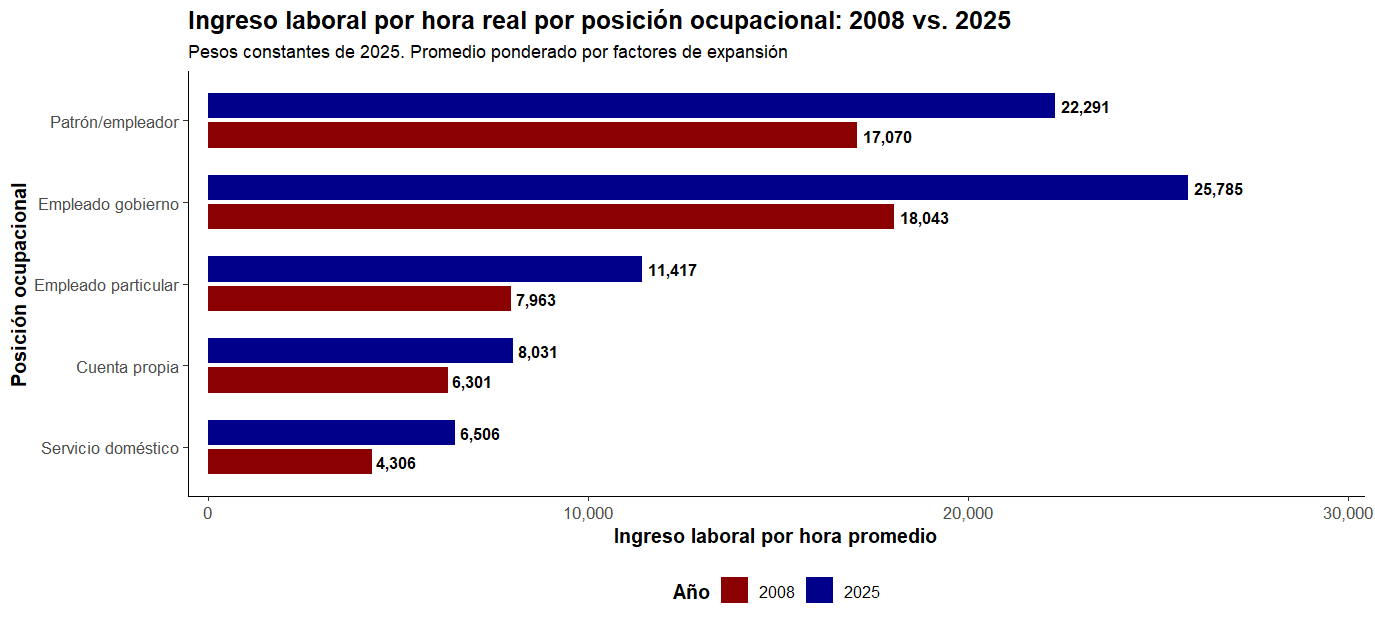
\includegraphics[width=0.9\textwidth]{Paper/figures/fig7Informe.png}
  \caption{Ingreso laboral por posición ocupacional}
  \label{fig:3Informe}
\end{figure}

La posición que ocupa un trabajador dentro del mercado laboral también hace una diferencia enorme. En 2025, los empleados del gobierno son quienes mejor ganan (\$25.785 por hora), seguidos por los patrones o empleadores (\$22.291). En el extremo opuesto, los trabajadores domésticos y los cuenta propia tienen los ingresos más bajos, aunque todos los grupos muestran mejoras reales frente a 2008.
Un dato destacado es el crecimiento del servicio doméstico: pasó de \$4.306 a \$6.506, un incremento de más del 50\% en términos reales. Esto posiblemente esté relacionado con los ajustes en la regulación laboral y los aumentos acumulados del salario mínimo durante el período.

\begin{figure}[htbp]
  \centering
  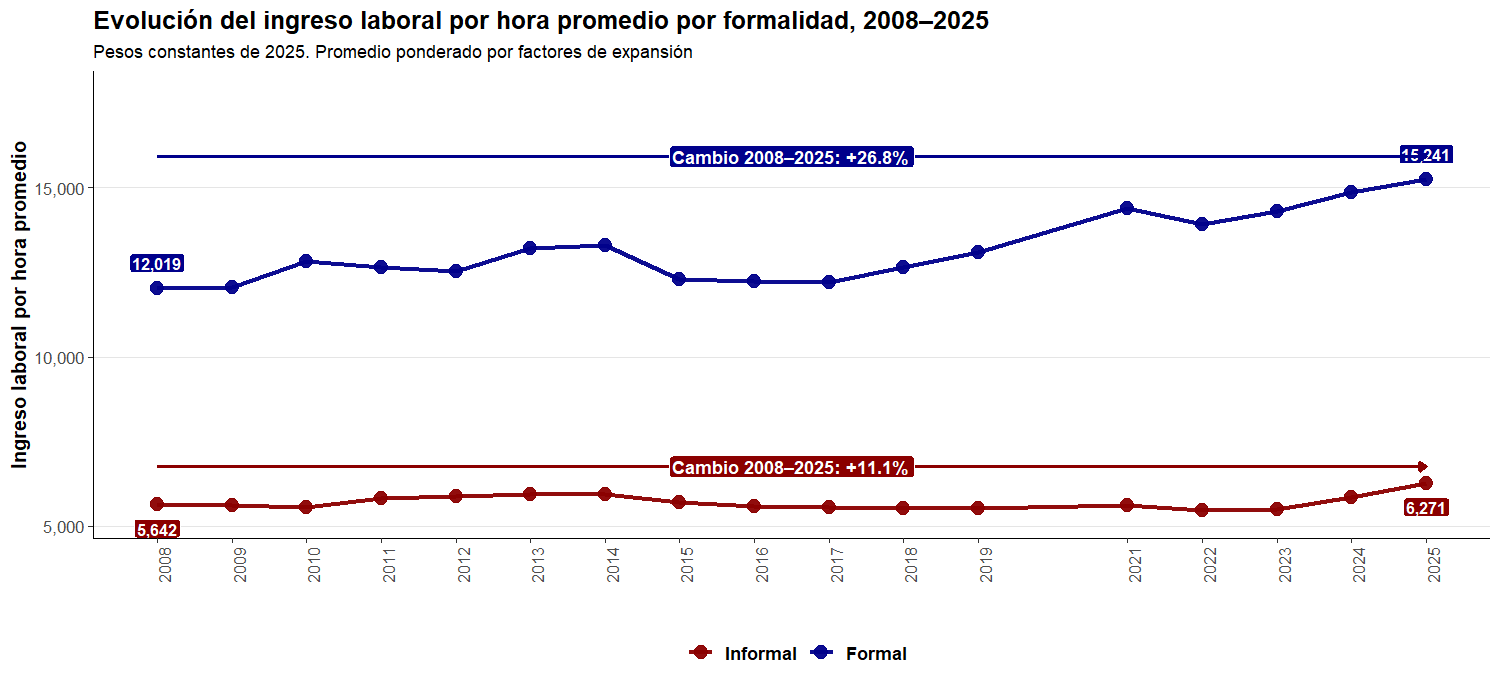
\includegraphics[width=0.9\textwidth]{Paper/figures/fig4Informe.png}
  \caption{Ingreso laboral por formalidad}
  \label{fig:4Informe}
\end{figure}

\begin{figure}[htbp]
  \centering
  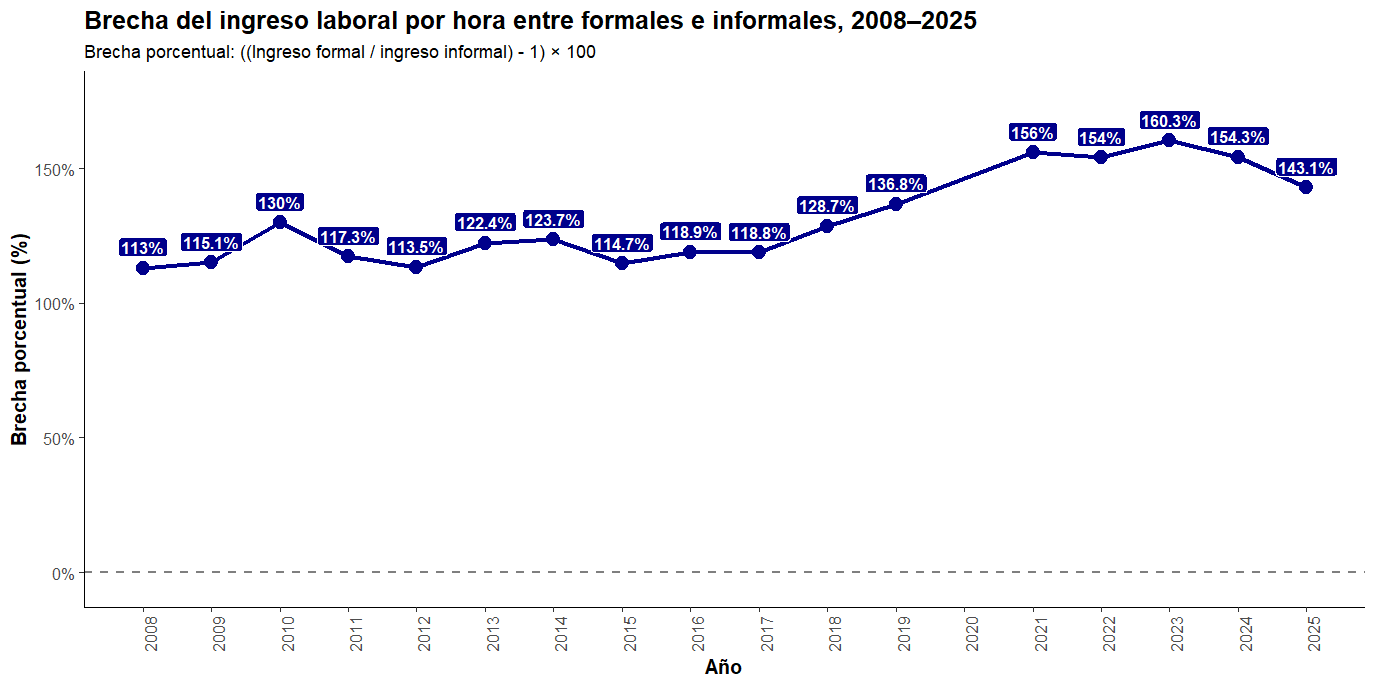
\includegraphics[width=0.9\textwidth]{Paper/figures/fig5Informe.png}
  \caption{Brecha por formalidad}
  \label{fig:5Informe}
\end{figure}

Esta es quizás una de las brechas más persistentes del mercado laboral colombiano. En 2025, un trabajador formal gana en promedio \$15.241 por hora, mientras que uno informal gana apenas \$6.271. Eso significa que los formales ganan aproximadamente 143\% más que los informales, una brecha que además ha crecido a lo largo del período (era del 113\% en 2008).
Aunque el ingreso de los informales sí creció en términos reales (+11,1\%), lo hizo mucho más lentamente que el de los formales (+26,8\%). Esto sugiere que la formalización laboral no solo importa para el acceso a seguridad social, sino también para el nivel de ingresos.

\begin{figure}[htbp]
  \centering
  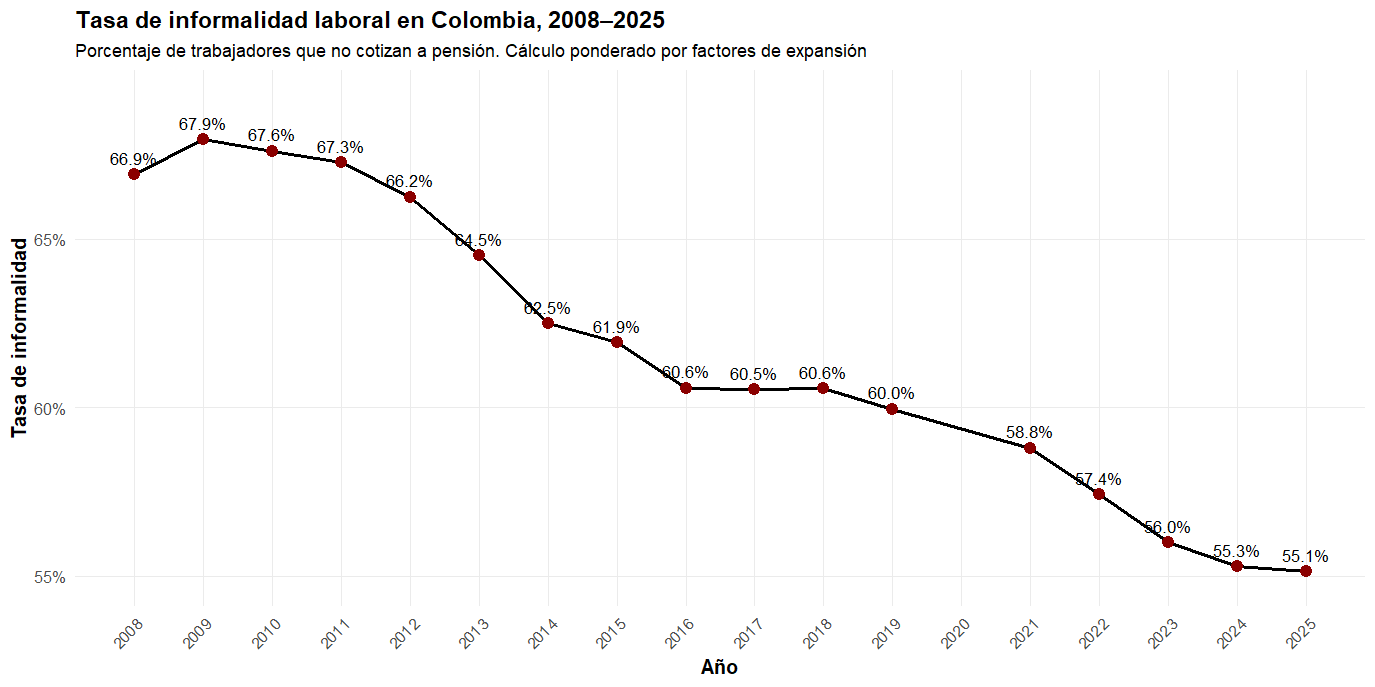
\includegraphics[width=0.9\textwidth]{Paper/figures/fig11Informe.png}
  \caption{Evolución informalidad laboral}
  \label{fig:6Informe}
\end{figure}

En cuanto a la tasa de informalidad, hay una tendencia positiva: bajó del 66,9\% en 2008 al 55,1\% en 2025. Una reducción de casi 12 puntos porcentuales en 17 años es significativa, aunque el nivel sigue siendo muy alto. Más de la mitad de los trabajadores colombianos aún no cotiza a pensión.

\begin{figure}[htbp]
  \centering
  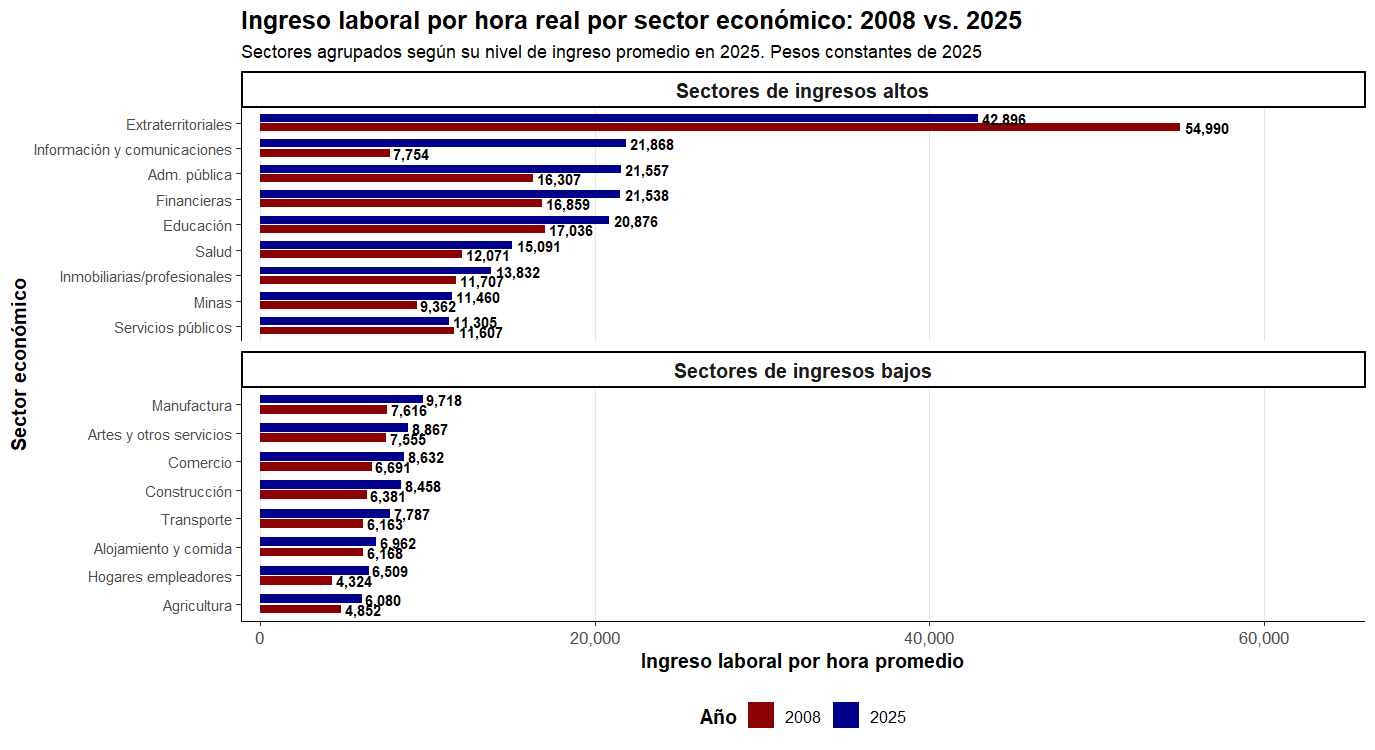
\includegraphics[width=0.9\textwidth]{Paper/figures/fig9Informe.png}
  \caption{Ingreso laboral por sector económico}
  \label{fig:7Informe}
\end{figure}

Existe una marcada división entre sectores de altos y bajos ingresos. En la parte alta se encuentran los sectores extraterritoriales, información y comunicaciones, administración pública, financiero y educación. En la parte baja, sectores como agricultura, hogares empleadores, alojamiento y construcción.
El sector de información y comunicaciones es el que más creció: casi triplicó su ingreso real entre 2008 y 2025 (de \$7.754 a \$21.868). Esto refleja la expansión de la economía digital y la creciente demanda de talento tecnológico, y es una señal clara de hacia dónde apunta el futuro del trabajo en Colombia.
La agricultura, por su parte, sigue siendo el sector de menores ingresos, con apenas \$6.080 por hora en 2025.

\begin{figure}[htbp]
  \centering
  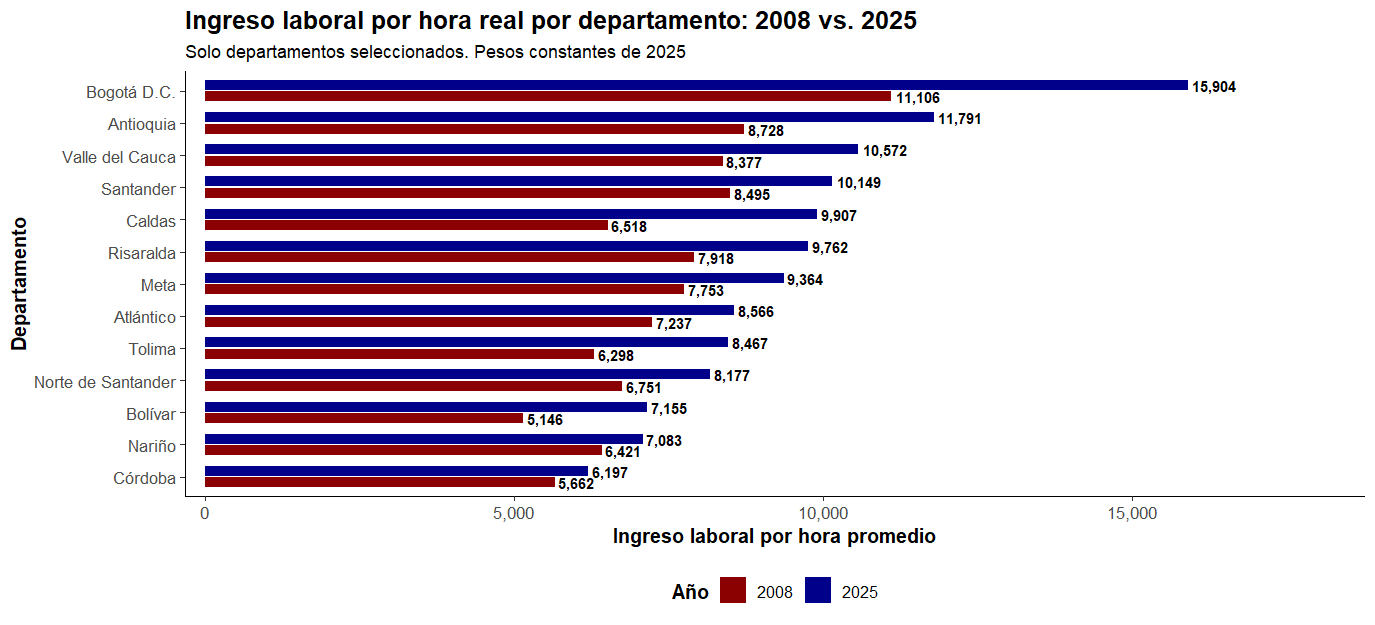
\includegraphics[width=0.9\textwidth]{Paper/figures/fig8Informe.png}
  \caption{Ingreso laboral por departamento}
  \label{fig:8Informe}
\end{figure}

Las brechas regionales son evidentes. Bogotá D.C. lidera con un ingreso promedio de \$15.904 por hora en 2025, seguida por Antioquia (\$11.791) y Valle del Cauca (\$10.572). En el extremo opuesto, departamentos como Córdoba, Nariño y Bolívar tienen los ingresos más bajos, aunque todos registraron ganancias reales frente a 2008.
Un dato interesante es que Caldas muestra uno de los mayores crecimientos proporcionales del período, lo que podría estar relacionado con su dinámica agroindustrial y de servicios. Las brechas entre el centro del país y las regiones periféricas persisten y son un desafío estructural importante.

\newpage
\begin{figure}[htb]
  \centering
  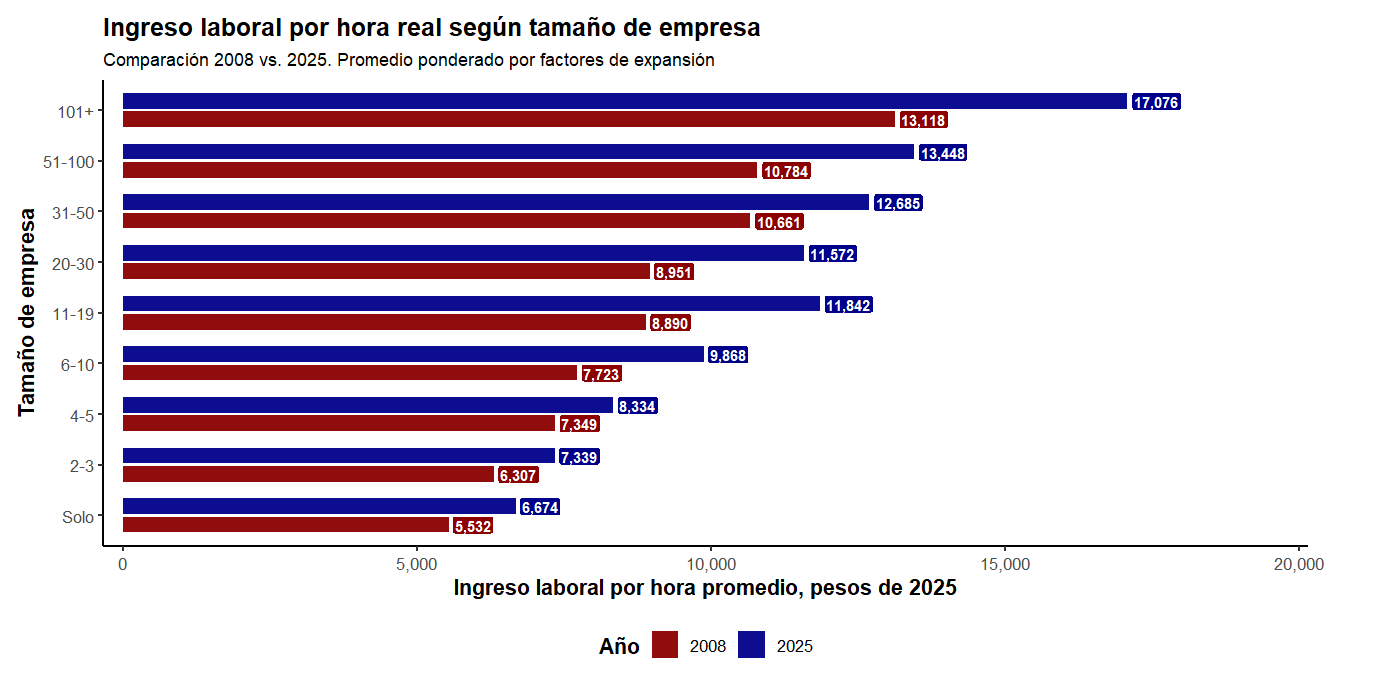
\includegraphics[width=0.9\textwidth]{Paper/figures/fig10Informe.png}
  \caption{Ingreso laboral por tamaño de empresa}
  \label{fig:9Informe}
\end{figure}

Como era de esperarse, las empresas más grandes pagan mejor. En 2025, las empresas de más de 100 empleados ofrecen un ingreso promedio de \$17.076 por hora, mientras que los trabajadores que laboran solos apenas alcanzan \$6.674.
Hay además un cambio estructural relevante entre 2008 y 2025: la participación del empleo en empresas muy pequeñas (solo y 2-3 personas) cayó, mientras que la de las empresas grandes (101+) aumentó del 19\% al 25\%. Esto podría ser una señal positiva de consolidación empresarial, aunque también puede reflejar la formalización de sectores que antes operaban en la informalidad.

\begin{figure}[htb]
  \centering
  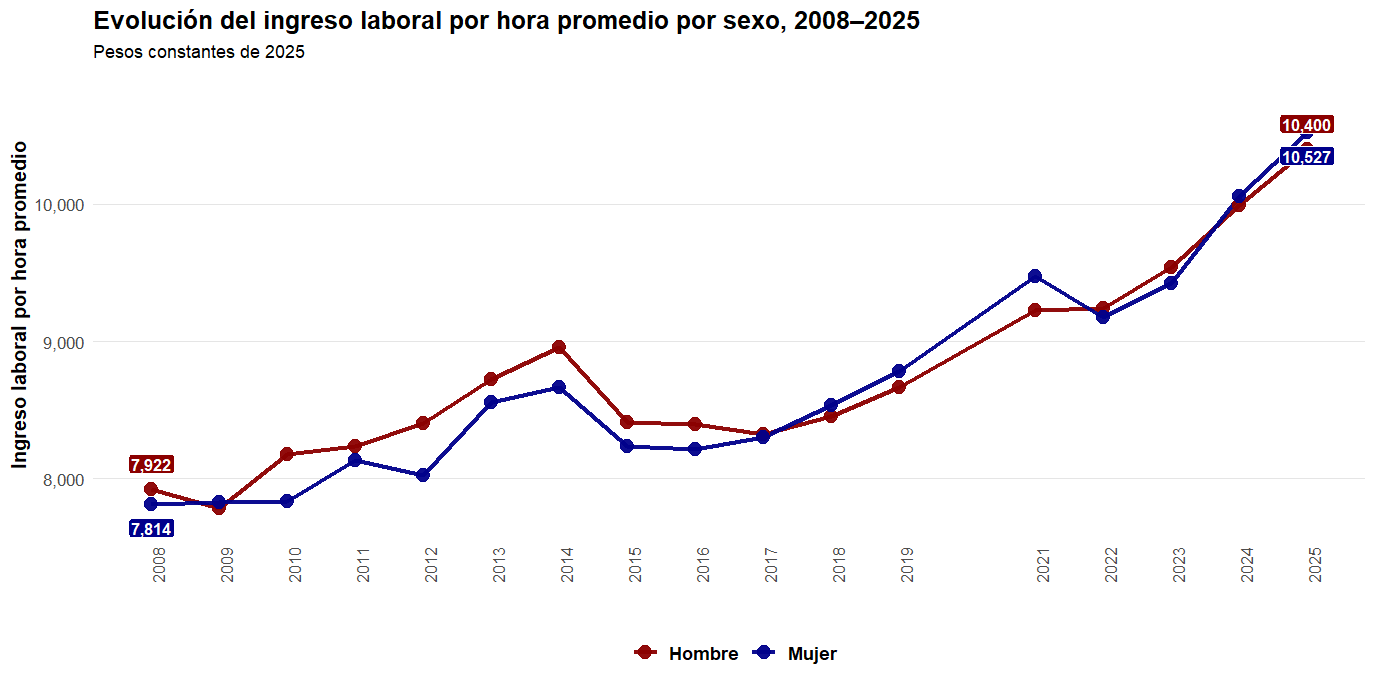
\includegraphics[width=0.9\textwidth]{Paper/figures/fig2Informe.png}
  \caption{Brecha de género}
  \label{fig:10Informe}
\end{figure}

\begin{figure}[htb]
  \centering
  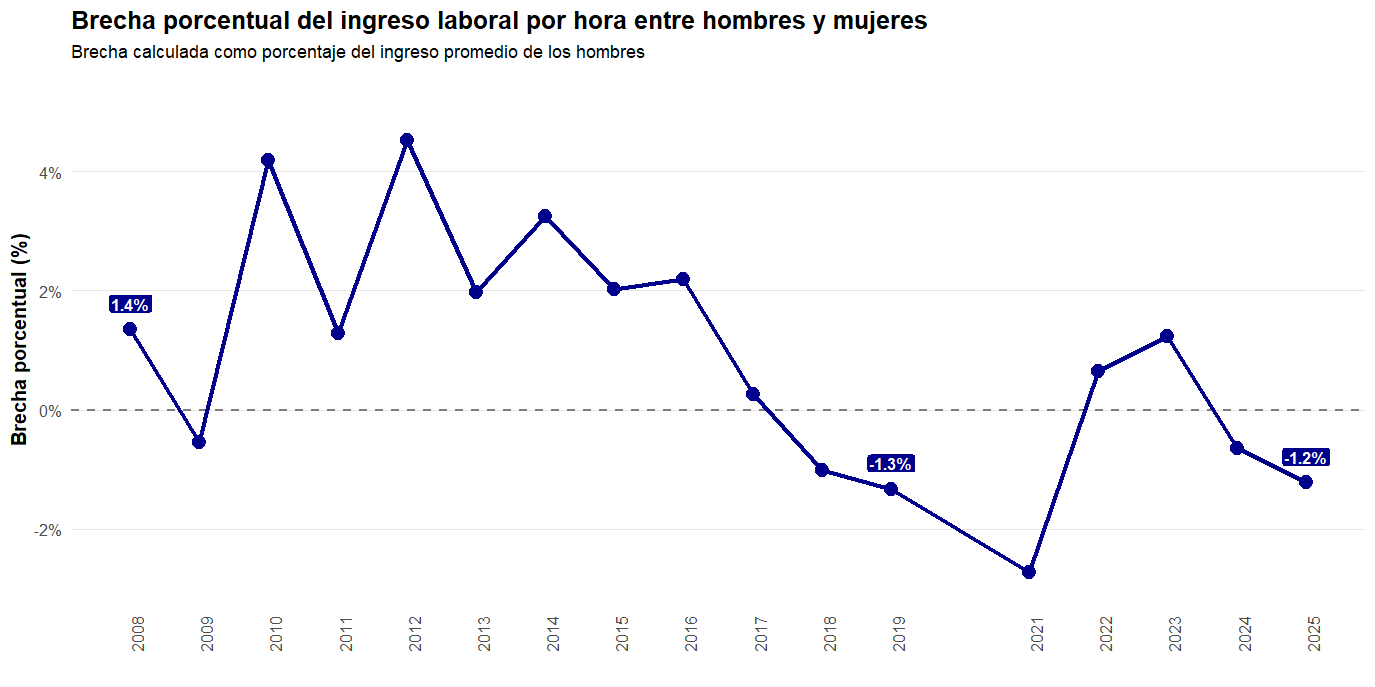
\includegraphics[width=0.9\textwidth]{Paper/figures/fig3Informe.png}
  \caption{Brecha de género porcentual}
  \label{fig:11Informe}
\end{figure}

Una de las noticias más llamativas del período es la evolución de la brecha salarial por género. En 2008, los hombres ganaban en promedio un 1,4\% más que las mujeres por hora. Para 2025, esa relación se invirtió: las mujeres ganan un 1,2\% más que los hombres.

\section{Conclusión}
El mercado laboral colombiano entre 2008 y 2025 muestra un panorama de progreso real pero desigual. Los ingresos crecieron en términos generales, la informalidad bajó y la brecha de género prácticamente desapareció. Esas son ganancias concretas que no deben subestimarse.

Sin embargo, persisten desafíos estructurales importantes. La brecha entre trabajadores formales e informales se amplió. Las diferencias regionales siguen siendo grandes. Y aunque todos los sectores mejoraron, los trabajadores en actividades de baja productividad, como agricultura o trabajo doméstico, siguen muy lejos de los ingresos del resto.

La historia que cuentan estas cifras es la de un mercado laboral que avanza, pero que aún tiene una deuda pendiente con millones de trabajadores que, pese a trabajar, no acceden a condiciones laborales dignas ni a los beneficios de la seguridad social.